%%%%%%%%%%%%%%%%%%%%%%%%%%%%%%%%%%%%%%%%%%%%%%%%%%%%%%%%%%%%%%%%%%%%%%%%
%                                                                      %
%     File: Thesis_ActiveSolution.tex                                  %
%     Tex Master: Thesis.tex                                           %
%                                                                      %
%     Author: Miguel Fonseca                                           %
%     Last modified : 8 Jul 2015                                       %
%                                                                      %
%%%%%%%%%%%%%%%%%%%%%%%%%%%%%%%%%%%%%%%%%%%%%%%%%%%%%%%%%%%%%%%%%%%%%%%%

\chapter{Infrared Solution}
\label{chapter:active}
As there is still no global procedure to register UA, the use of unique identification for a sense and avoid system should be averted. It is important to notice that, in order to prevent collisions, the specific knowledge of the intruder's identification is not required. Only the type of aircraft is required so that right-of-way rules may be applied.\\
The proposed sense and avoid system should not be expensive to allow easy access for the owners of cheap small unmanned aircraft. It is also important to use small and lightweight equipment/materials that is readily available from local electronics stores or websites, so that its implementation has a good cost/benefit relation.\\
Finally, the system should provide detection as well as relative position between multiple unmanned aircraft, to enable collision avoidance by corrections of the original flight path.\\

\section{Choosing the solution}
\label{section:choosing}
\subsection{Electromagnetic spectrum's frequency}
\label{subsection:eospectrum}
In order to use a wireless cooperative system, an operating frequency from the electromagnetic spectrum, depicted in figure \ref{fig:spectrum}, has to be chosen.
\begin{figure}[!htb]
  \centering
  \includegraphics[width=0.8\textwidth]{Figures/spectrum.png}
  \caption[Electromagnetic Spectrum \citep{Haynes}]{Electromagnetic Spectrum \citep{Haynes}}
  \label{fig:spectrum}
\end{figure}
\subsubsection{Radio and Micro waves}
The radio and microwaves' spectrum are highly regulated and usually require a permit for operation. This area of the electromagnetic spectrum is already highly used in many different technologies in aviation, such as ADS-B and TCAS, or for common use, like radio and television, among others. This type of technology generally requires high power equipment to transmit the signal, which sUA cannot provide due to their low power batteries.\\
To avoid using high power equipment in the aircraft, it is possible to use a network of communication already in use, such as the GSM network. This type of network allows the user to operate with small, low power equipment, using instead several fixed antennas with high gain to provide the required coverage. This solution has several problems however. Because the aircraft would depend on fixed equipment and omni-directional antennas for communication, it is harder to compute the aircraft's localization: one way to do this is triangulation, which requires the aircraft to be in range of several antennas; and another way is for the aircraft to use another source of localization, such as GNSS, which has been hacked in the past \citep{Emspak2011} \citep{BBCNewsTechnology2012} and may provide errors in GPS denied areas. Adding to this, each aircraft would be required to have a unique identification and, as there is still no international standard, it is impossible to ask for it at this time. Using the same network as cellphone users would have other problems: for example, during certain events, the GSM network is not able to withstand the number of users, which would deprive an aircraft of its main sense and avoid system.\\
\subsubsection{Visible, Ultraviolet and higher frequency waves}
Ultraviolet (UV) waves interact with the Earth's atmosphere by scattering. Although this facilitates their propagation under non-line-of-sight communications, it would not be ideal to provide relative position \citep{Cruz}.\\
Frequencies above the UV spectrum, such as x-rays and gamma rays, may have several risks for human health due to their high levels of energy \citep{Waltz2008}. \\
Visual light spectrum has too much ambient noise, as can be seen in figure \ref{fig:solarspectrum}, which requires high processing capabilities to enable detection.\\
\subsubsection{Infrared spectrum}
The remaining Infrared waves may have wavelengths between 750 nm to 1 mm (or frequencies from 400 THz to 300 GHz). The International Commission on Illumination (CIE) divides the infrared radiation in three different sections: IR-A (0.78 $\mu$m to 1.4 $\mu$m), IR-B (1.4 $\mu$m to 3 $\mu$m) and IR-C (3 $\mu$m to 1000 $\mu$m) \citep{Taylor2000}. \\
Although there are some reported cases of humans being able to see the lower wavelength infrared \citep{Cox}, the majority is not able to see above wavelengths of 780 nm , which means that using an infrared wave for communication purposes does not create visual pollution.\\
Adding to this, the infrared spectrum is unregulated \citep{Hou2015}, except for health concerns \citep{Ghassemlooy2006}, and it is not necessary a license to operate in these frequencies \citep{Hou2015}. Although there is still some infrared radiation from the sun that reaches the sea level, a large percentage is filtered by the atmosphere, particularly in some wavelengths due to the interaction with molecules such as O$_{2}$ and H$_{2}$O, as can be seen in figure \ref{fig:solarspectrum}.\\
\begin{figure}[!htb]
  \centering
  \includegraphics[width=0.70\textwidth]{Figures/SolarSpectrum.png}
  \caption[Solar Radiation Spectrum \citep{Rohde2007}]{Solar Radiation Spectrum \citep{Rohde2007}}
  \label{fig:solarspectrum}
\end{figure}

Another important advantage is that, by using a completely different wavelength than other communication systems used in aviation, such as TCAS and ADS-B, the proposed system is transparent to them. This means that an infrared communication system cannot interfere with the systems in operation nowadays, with the downside of not being able to receive and cooperate with them.\\
Because the infrared waves have a behavior much different from radio and microwaves, it does not generate radio-frequency interference (RFI), which is known for creating disturbances in electrical circuits due to electromagnetic radiation or electromagnetic induction \citep{Hou2015}. This is essential in a system that operates in close proximity to the autopilot or flight management system of an aircraft through cable communications.\\

Despite this, there are several problems with IR-B and IR-C frequencies. There is too much noise generated by objects and animals on the Earth's surface to use IR-C. Adding to this, the atmosphere has poor transmission on wavelengths between 5 to 8 $\mu$m \citep{Cox}. Finally, the typical used silicon photodiodes are not sensitive above 1100 nm \citep{Ryer.1998} which turns the IR-B frequencies expensive to work with.\\

The IR-A wavelengths also have some disadvantages. The main disadvantage is its range: IR signals may be adversely affected by dust, scintillation, smoke and some weather conditions \citep{Pauluzzi1992}. Weather conditions, such as fog, rain and snow, can generate different amounts of attenuation: depending on its density, fog can decrease the range of communication from 30 m in a clear day down to 7.5 m, with a total attenuation of 12 dB \citep{Pauluzzi1992}. For comparison, heavy rain would only decrease the same signal to 28 m, with an even smaller decrease generated by dust and snow \citep{Pauluzzi1992}. Scintillation, which is a fluctuation in the refraction index of the air due to uneven heating of air, may cause a reduction in range to half the original value \citep{Pauluzzi1992}.\\ 
The fact that IR waves cannot penetrate walls has the disadvantage of creating zones where the signal doesn't reach. Because of this, a sense and avoid system that uses the infrared spectrum may present poor results in places with big obstacles, such as cities and mountains, or indoors: if an intruder is located behind an obstacle, it will not be detected until both aircraft are too close. Adding to this, because infrared waves reflect in several surfaces, there is also the danger of multipaths and the risk of aircraft receiving its own signal. Multipaths may generate inter-symbol interference \citep{Ghassemlooy2006} or, in the specific case in study, the illusion of an aircraft in a position that is not correct, while an aircraft receiving its own signal will detect an aircraft that does not exist.\\ 
As UV waves, the infrared spectrum can also pose a risk to human health, specially to the eyes. This risk is minimized when using LEDs as the source of infrared waves, instead of lasers which have a much more concentrated beam \citep{Ghassemlooy2006}. There is also risk to the skin but this requires power levels much higher than for the eyes. Finally, long-term exposure to IR waves is negligible, as the ambient light sources are constantly submitting our bodies to much higher radiation levels than the studied systems \citep{Kahn1997}. Even so, the risk for human health must be accounted for when selecting the material for the prototype.\\

In the IR-A, or near infrared, there could be several wavelength options. O$_{2}$ has a significant impact in filtering the Sun's radiation with 0.76 $\mu$m of wavelength without reducing its transmission too much. H$_{2}$O has a similar effect for radiation with wavelength around 0.72 $\mu$m, 0.82 $\mu$m, 0.94 $\mu$m and 1.1 $\mu$m \citep{Cox} \citep{Cornelius}.\\
The available wide bandwith at this range (200 THz in the 700-1500 nm range) \citep{Ghassemlooy2006} cannot penetrate walls, which decreases significantly the probability of interfering with other applications that use infrared waves \citep{Pauluzzi1992}, such as remote controls.\\
The 940/950 nm wavelength is broadly used in remote controls which means that emitters and receivers have a very low cost market \citep{Hou2015} \citep{Rao2013}, which is highly desirable.\\

There are two main sources used to transmit infrared radiation in the 940/950 nm wavelength: Lasers and LEDs. Although lasers have broader bandwidth, the acquisition costs are higher \citep{Pauluzzi1992} and they have several restrains due to eye safety issues \citep{Ghassemlooy2006}, as previously discussed. LEDs have relaxed eye safety due to the dispersion of power through the wider angular beam. Adding to this, the laser's smaller angular beam would not be appropriate to provide the required angular coverage.
\subsection{Communication Type}
\label{subsection:communication}
As in chapter \ref{chapter:passive}, the proposed system uses an approach similar to a solution already used in aviation. \\
The Very High Frequency Omni-directional Range (VOR) is a conventional radio navigation aid which encodes the azimuth as the relation between two modulations: reference and variable phase modulations \citep{InternationalCivilAviationOrganization2006}. The difference between the two signals' phases is equal to the angle between the magnetic north and the receiver. This enables the pilot of an aircraft to know his position relative to the VOR.\\
The proposed system replaces the radio signals with IR transmitting LEDs and the phase difference with a communication protocol. To avoid moving parts, several transmitting sectors will be designed, each with one LED, as well as different reception sectors, each with one receiver. The number of LEDs and receivers must be enough to cover all horizontal 360\degree, without overlapping, either for transmission and reception. The relative position will be given by the number of the receiver and by the information sent by each LED. This way, the aircraft can compute the intruders direction and predict a possible collision.\\
Adding to this, the transmitted message will contain the transmitting aircraft's type, so that right-of-way rules can be applied.\\

Consumer IR is the utilization of infrared for communication between consumer electronics. The near-infrared band, or IR-A, is always used so that cheap PIN diodes can be used as receivers. IR receivers used in consumer electronics usually have a preamplifier and a package which behaves as an IR filter \citep{Vishay2013}. To distinguish the signal from the ambient noise, the signal is modulated at a predetermined frequency, usually between 30 and 60 kHz, by turning the carrier on and off (Pulse Width Modulation or PWM). Also because of ambient generated noise, the receivers are adapted for short bursts of communication which contain information encoded into bits \citep{Vishay2013}. 
Although there are many different consumer IR protocols, the most used are Philips' RC-5 and RC-6, the Japanese NEC and the SONY's SIRC. The adopted one was the RC-5, due to the available knowledge about the correct timings and structure of the code, as listed in figure \ref{fig:rc5protocol}.\\
\begin{figure}[!htb]
  \centering
  \includegraphics[width=0.9\textwidth]{Figures/rc5protocol.jpg}
  \caption[RC5-5 Philips Protocol details \citep{Infrarossidotit2009}]{RC5-5 Philips Protocol details \citep{Infrarossidotit2009}}
  \label{fig:rc5protocol}
\end{figure}

As can be seen in figure \ref{fig:rc5protocol}, the RC-5 protocol uses bi-phase modulation (or Manchester code), where each data bit is coded into a sequence of lows and highs with the same duration: a '0' is represented by a high followed by a low, while a '1' is the inverse. The Manchester coding has several benefits, among which \citep{Pauluzzi1992}:
\begin{itemize}
\item "The power spectral density of the signal is shifted away from DC which helps to reduce low frequency (power line) interference, and it also eliminates baseband wander at the receiver."
\item "clock recovery is made simple since there is a logic transition in the center of every bit interval"
\item duty cycle of 50\% for bits 0 and 1
\end{itemize}
To avoid interference with consumer electronics, such as televisions, instead of using the standard 36 kHz modulation, a higher frequency of 56 kHz will be used. As can be seen in figure \ref{fig:receiverfrequency}, the responsivity of a 36 kHz receiver for a 56 kHz modulated signal is under 0.2.\\
\begin{figure}[!htb]
  \centering
  \includegraphics[width=0.7\textwidth]{Figures/receiverfrequency.png}
  \caption[IR Receiver TSOP48's Frequency Dependence of Responsivity \citep{Vishay2015}]{IR Receiver TSOP48's Frequency Dependence of Responsivity \citep{Vishay2015}}
  \label{fig:receiverfrequency}
\end{figure}

As the RC-5 has a PWM modulation as well as the Manchester coding, the duty cycle decreases to 25\% , which is desired to reduced the battery's toll.\\

The original RC-5 signal, as can be seen in figure \ref{fig:rc5protocol}, is composed by:
\begin{itemize}
\item 2 start bits
\item 1 toggle bit
\item 5 bits to represent the IR device address
\item 6 bits with the command
\end{itemize} 


\subsection{Proposed Solution}
\label{subsection:solution}
The proposed solution, as seen in figure \ref{fig:irdiagram}, uses 16 transmitting sectors, each with one IR LED with an angle of half transmission equal to 20\degree , located all around the prototype and 4 receiving sectors, each with one IR receiver with an angle of half transmission equal to 90\degree , located at the center so that no overlapping can happen in the reception.\\
\begin{figure}[!htb]
  \centering
  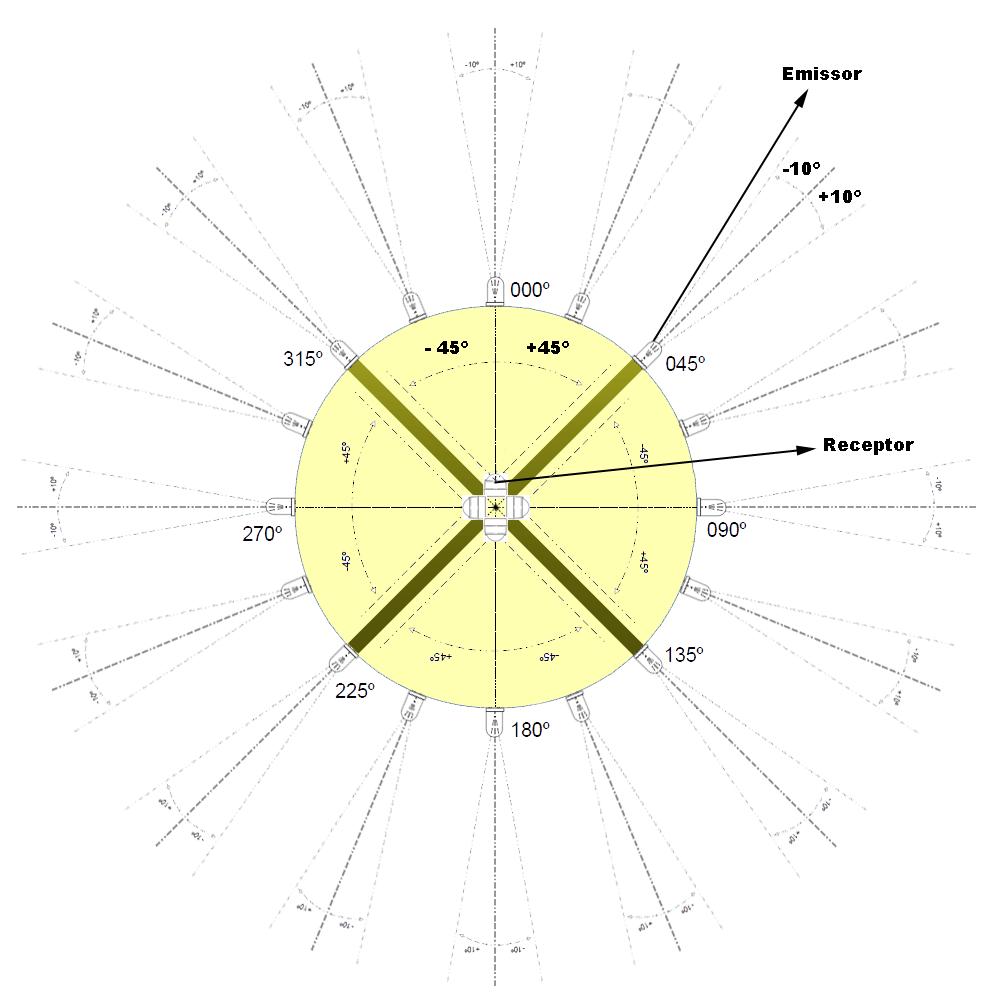
\includegraphics[width=0.8\textwidth]{Figures/esquemaIR16.png}
  \caption[IR diagram]{IR diagram}
  \label{fig:irdiagram}
\end{figure}

Because the PWM modulation frequency has been changed, the address bits are no longer necessary and so the available 5 bits will be used to transmit the aircraft's category. Adding to this, as the prototype only requires 16 transmitting sectors, we only need 4 bits to send their identification. And so, the transmitted message will be composed by:
\begin{itemize}
\item 2 start bits
\item 1 toggle bit
\item 5 bits to represent the type of aircraft
\item 4 bits with sector identification
\end{itemize} 
With this, the transmitted signal is shorter than the standard RC-5, which will enable an increase in the transmission rate.\\

The prototype will only handle the sensing of intruders, as the tracking and collision avoidance may require more processing power than an Arduino\texttrademark board can offer. After receiving a signal, the Arduino\texttrademark board should send it to the autopilot, which is then responsible to determine if any measures are necessary to avoid collision and which maneuvers should be applied.\\

\section{Material}
\label{section:material}
To enable the requirements cited in the previous section, the material will be chosen from websites from local electronics stores. The required materials are shown in figure \ref{fig:irblockdiagram}.\\
\begin{figure}[!htb]
  \centering
  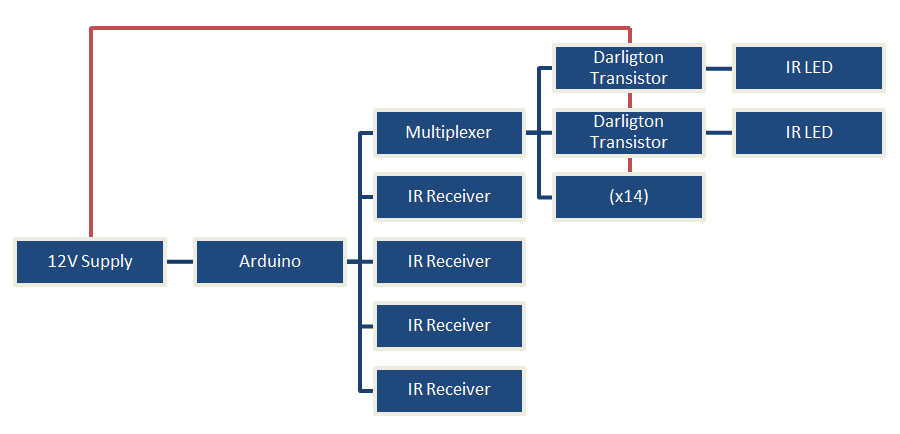
\includegraphics[width=0.8\textwidth]{Figures/blocoscompleto.png}
  \caption[Block Diagram of the IR Anti-Collision System]{Block Diagram of the IR Anti-Collision System}
  \label{fig:irblockdiagram}
\end{figure}

The Arduino\texttrademark board was chosen according to the AHP already explained in section \ref{subsection:arduinoAHP}. The Arduino\texttrademark Pro Mini is responsible for controlling the transmission by the LEDs as well as the reception by the receivers.\\
Most Arduino\texttrademark boards can only perform one task at a time. Because of this, the prototype will only be able to transmit or receive at any given time, and the transmission can only happen in one LED at a time, as each LED will transmit a different message which identifies its sector.\\
As the used signal uses a modulation of 56 kHz which can only be generated to one pin of the Arduino\texttrademark board, and the prototype is designed to employ 16 sectors with one LED per sector as well as 4 receivers, and an Anti-collision light from chapter \ref{chapter:passive}, and the Arduino\texttrademark Pro Mini only has 14 digital I/O Pins, we need to use a multiplexer to control all the LEDs.\\
The 74HC4067 16-channel analog multiplexer/demultiplexer was chosen to control the LEDs, allowing to control 16 LEDs and only using 5 control pins: one with the transmitted signal and four to select the correct LED. The acquisition cost is \euro{0.6}.\\
The selected multiplexer requires a supply voltage under 11 V, typically around 5 V, which the Arduino\texttrademark board can provide. At an operating voltage of 5 V, the propagation delay from input Z to the outputs Yn is between 6 and 18 nse. The fastest switch the prototype requires is related to the 56 kHz modulation, which corresponds to a switch every 17.9 $\mu$s. As the maximum switching time of the selected multiplexer is 18 ns, it can easily transmit the required signal. In order to save space, a small outline integrated circuit (SOIC) package will be used.\\

The prototype requires receivers with an angle of half transmission distance equal or higher than 90\degree, operating voltage equal to 5 V, internal preamplifier and filter for 56 kHz modulation, peak wavelength between 940 and 950 nm and filter of IR radiation.\\
The selected receiver is the Vishay TSOP4856 which is accessible in multiple online stores andprovides all the requirements \citep{Vishay2015}. The acquisition cost is \euro{1.7} per unit.\\ 

To select the required transmitter, knowing that the receiver's typical irradiance is equal to 0.12 mW/m$^{2}$ \citep{Vishay2015}, and using a minimum range of 40 m, we can approximate the required transmitter's radiant intensity using equation \ref{eq:radiant} \citep{Vishay}. The required minimum radiant intensity is equal to 192 mW/sr.\\
\begin{equation}\label{eq:radiant}
d=\sqrt{\frac{I_{e}}{E_{e}}}
\end{equation}
With:
\begin{itemize}
\item $d$ - range
\item $I_{e}$ - emitter intensity
\item $E_{e}$ - receiver irradiance
\end{itemize}
The transmitting LEDs must have a angle of half intensity equal to 20\degree , a peak wavelength between 940 and 950 nm and a radiant intensity above 192 mW/sr. \\
The selected transmitter is the Vishay TSAL6100 High Power Infrared Emitting Diode, with peak wavelength equal to 940 nm, angle of half intensity of $\pm$ 10\degree , which is designed for high pulse current operation as desired and has a radiant intensity above 300 mW/sr with a forward current of 200 mA, as can be seen in figure \ref{fig:ledintensity}. The IR LED has a rise and fall time of 15 ns. The acquisition cost is \euro{0.45}\\
\begin{figure}[!htb]
  \centering
  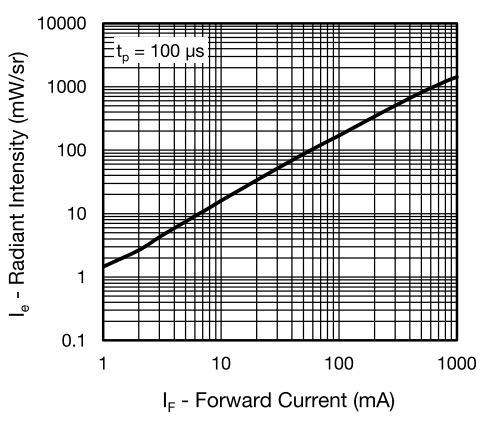
\includegraphics[width=0.6\textwidth]{Figures/ledintensity.png}
  \caption[TSAL6100 Radiant Intensity vs. Forward Current \citep{Vishay2014}]{TSAL6100 Radiant Intensity vs. Forward Current \citep{Vishay2014}}
  \label{fig:ledintensity}
\end{figure}
As the used LEDs require around 200 mA and the selected Arduino\texttrademark board can only provide up to 40 mA, a MOSFET or transistor is needed to control every LED with the Arduino. To avoid having 16 separate integrated circuits, an array should be used.\\
The selected transistor is the ULN2803A Darlington Transistor Array, which allows up to 500 mA peak collector current and an input voltage up to 30 V. Related to its switching characteristics, it has a propagation delay time of 130 ns for low to high level output and 20 ns for high to low level output, which is fast enough to generate the required 56 kHz modulation. In order to save space, a SOIC package will be used. The transistor in the selected package has an acquisition cost of \euro{0.8}.\\

To avoid oscillations due to the 56 kHz oscillation, as well as to protect the prototype from eventual peaks of tension from the source, a 1000 $\mu$F capacitor is going to be used, which has an acquisition cost of \euro{1.44}.\\

The LEDs' connections are illustrated in figure \ref{fig:IRlight}.\\
\begin{figure}[!htb]
  \centering
  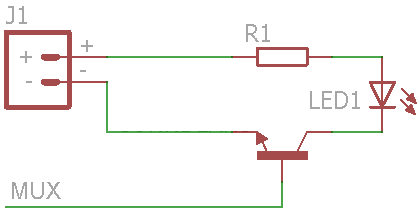
\includegraphics[width=0.4\textwidth]{Figures/EsquemasLights/IRlight.png}
  \caption[Diagram of the TSAL6100 and the ULN2803A Array connections]{Diagram of the TSAL6100 and the ULN2803A Array connections - the array is simplified into a single transistor}
  \label{fig:IRlight}
\end{figure}

As in section \ref{subsection:resistors}, the required resistances can be calculated in order to obtain the correct current in each LED, using easily available resistance values. Knowing that the aircraft used for testing uses a 3S battery (11.1V) and that, for the required forward current of 200 mA, the used LEDs have a forward voltage equal to 1.45 V, as can be seen in figure \ref{fig:irlightcurrent}, we can calculate the correct resistances.\\
\begin{figure}[!htb]
  \centering
  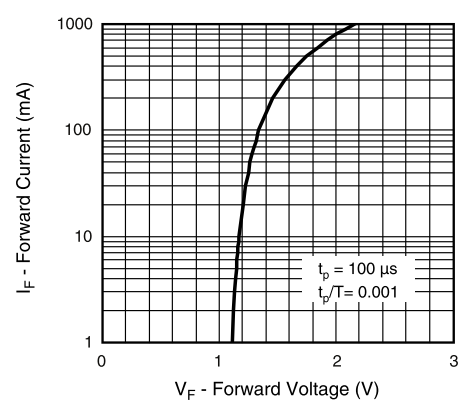
\includegraphics[width=0.6\textwidth]{Figures/irlightcurrent.png}
  \caption[TSAL6100 Forward Current vs Forward Voltage \citep{Vishay2014}]{TSAL6100 Forward Current vs Forward Voltage \citep{Vishay2014}}
  \label{fig:irlightcurrent}
\end{figure}

The voltage drop across each resistor can then be calculated according to equation \eqref{eq:voltagedrop2}.
\begin{equation}\label{eq:voltagedrop2}
V_{D}=V_{S}-V_{F}-V_{T}
\end{equation}
With:
\begin{itemize}
\item $V_{D}$ - Resistor's voltage drop
\item $V_{S}$ - source's voltage
\item $V_{F}$ - LED's forward voltage 
\item $V_{T}$ - Darlington Transistor Array forward voltage
\end{itemize}
According to figures~\ref{fig:IRlight}, the forward voltage for each component is equal to:
\begin{itemize}
\item IR LED - $V_{F} = 1.45 V$
\item ULN2803A Darlington Transistor Array - $V_{T} = 2 V$
\end{itemize}

The obtained value for the correct resistor's voltage drop is equal to 7.65 V. It is then possible to calculate the required resistance with Ohm's law, shown in equation \eqref{eq:ohm2}.
\begin{equation}\label{eq:ohm2}
R=\dfrac{V}{I}
\end{equation}
The obtained resistance is equal to 38.25 $\Omega$. Converting it to the nearest higher rated resistor, in order to use more available material while still protecting the LEDs from too much current, we get 39 $\Omega$. As in section \ref{chapter:passive}, the resistor has an acquisition cost of \euro{0.1}\\

\section{Software}
\label{section:software}

To transmit and receive information with IR frequencies, the IRremote library was adopted. Made by Ken Shirriff, this library allows communication using several IR protocols (such as NEC, Sony's SIRC, Philips RC-5 and RC-6, etc...) \citep{Shirriff2009}.
This library allows the configuration of an Arduino\texttrademark board as a transmitter or as a receiver, with pre-selected IR consumer protocol and frequency. It is also possible to configure the Arduino\texttrademark board as a receiver without specifying the protocol, receiving every signal sent in the receiver's frequency.\\
The IRremote library uses timers to control both the transmission and the reception. For transmission, the timer is programmed to generate PWM at the frequency required for the modulation. For reception, the timer is configured as an interrupt, running the reception code every 50 $\mu$s.\\

The transmitted message, as illustrated in figure \ref{fig:messagecode} is generated by first converting it to binary. This binary is then converted to the RC-5 protocol, with Manchester codification, by turning the timer that generates the PWM modulation on and off to create the necessary high levels and low levels of the message. Finally, the message is transmitted by the IR LEDs.\\
\begin{figure}[!htb]
  \centering
  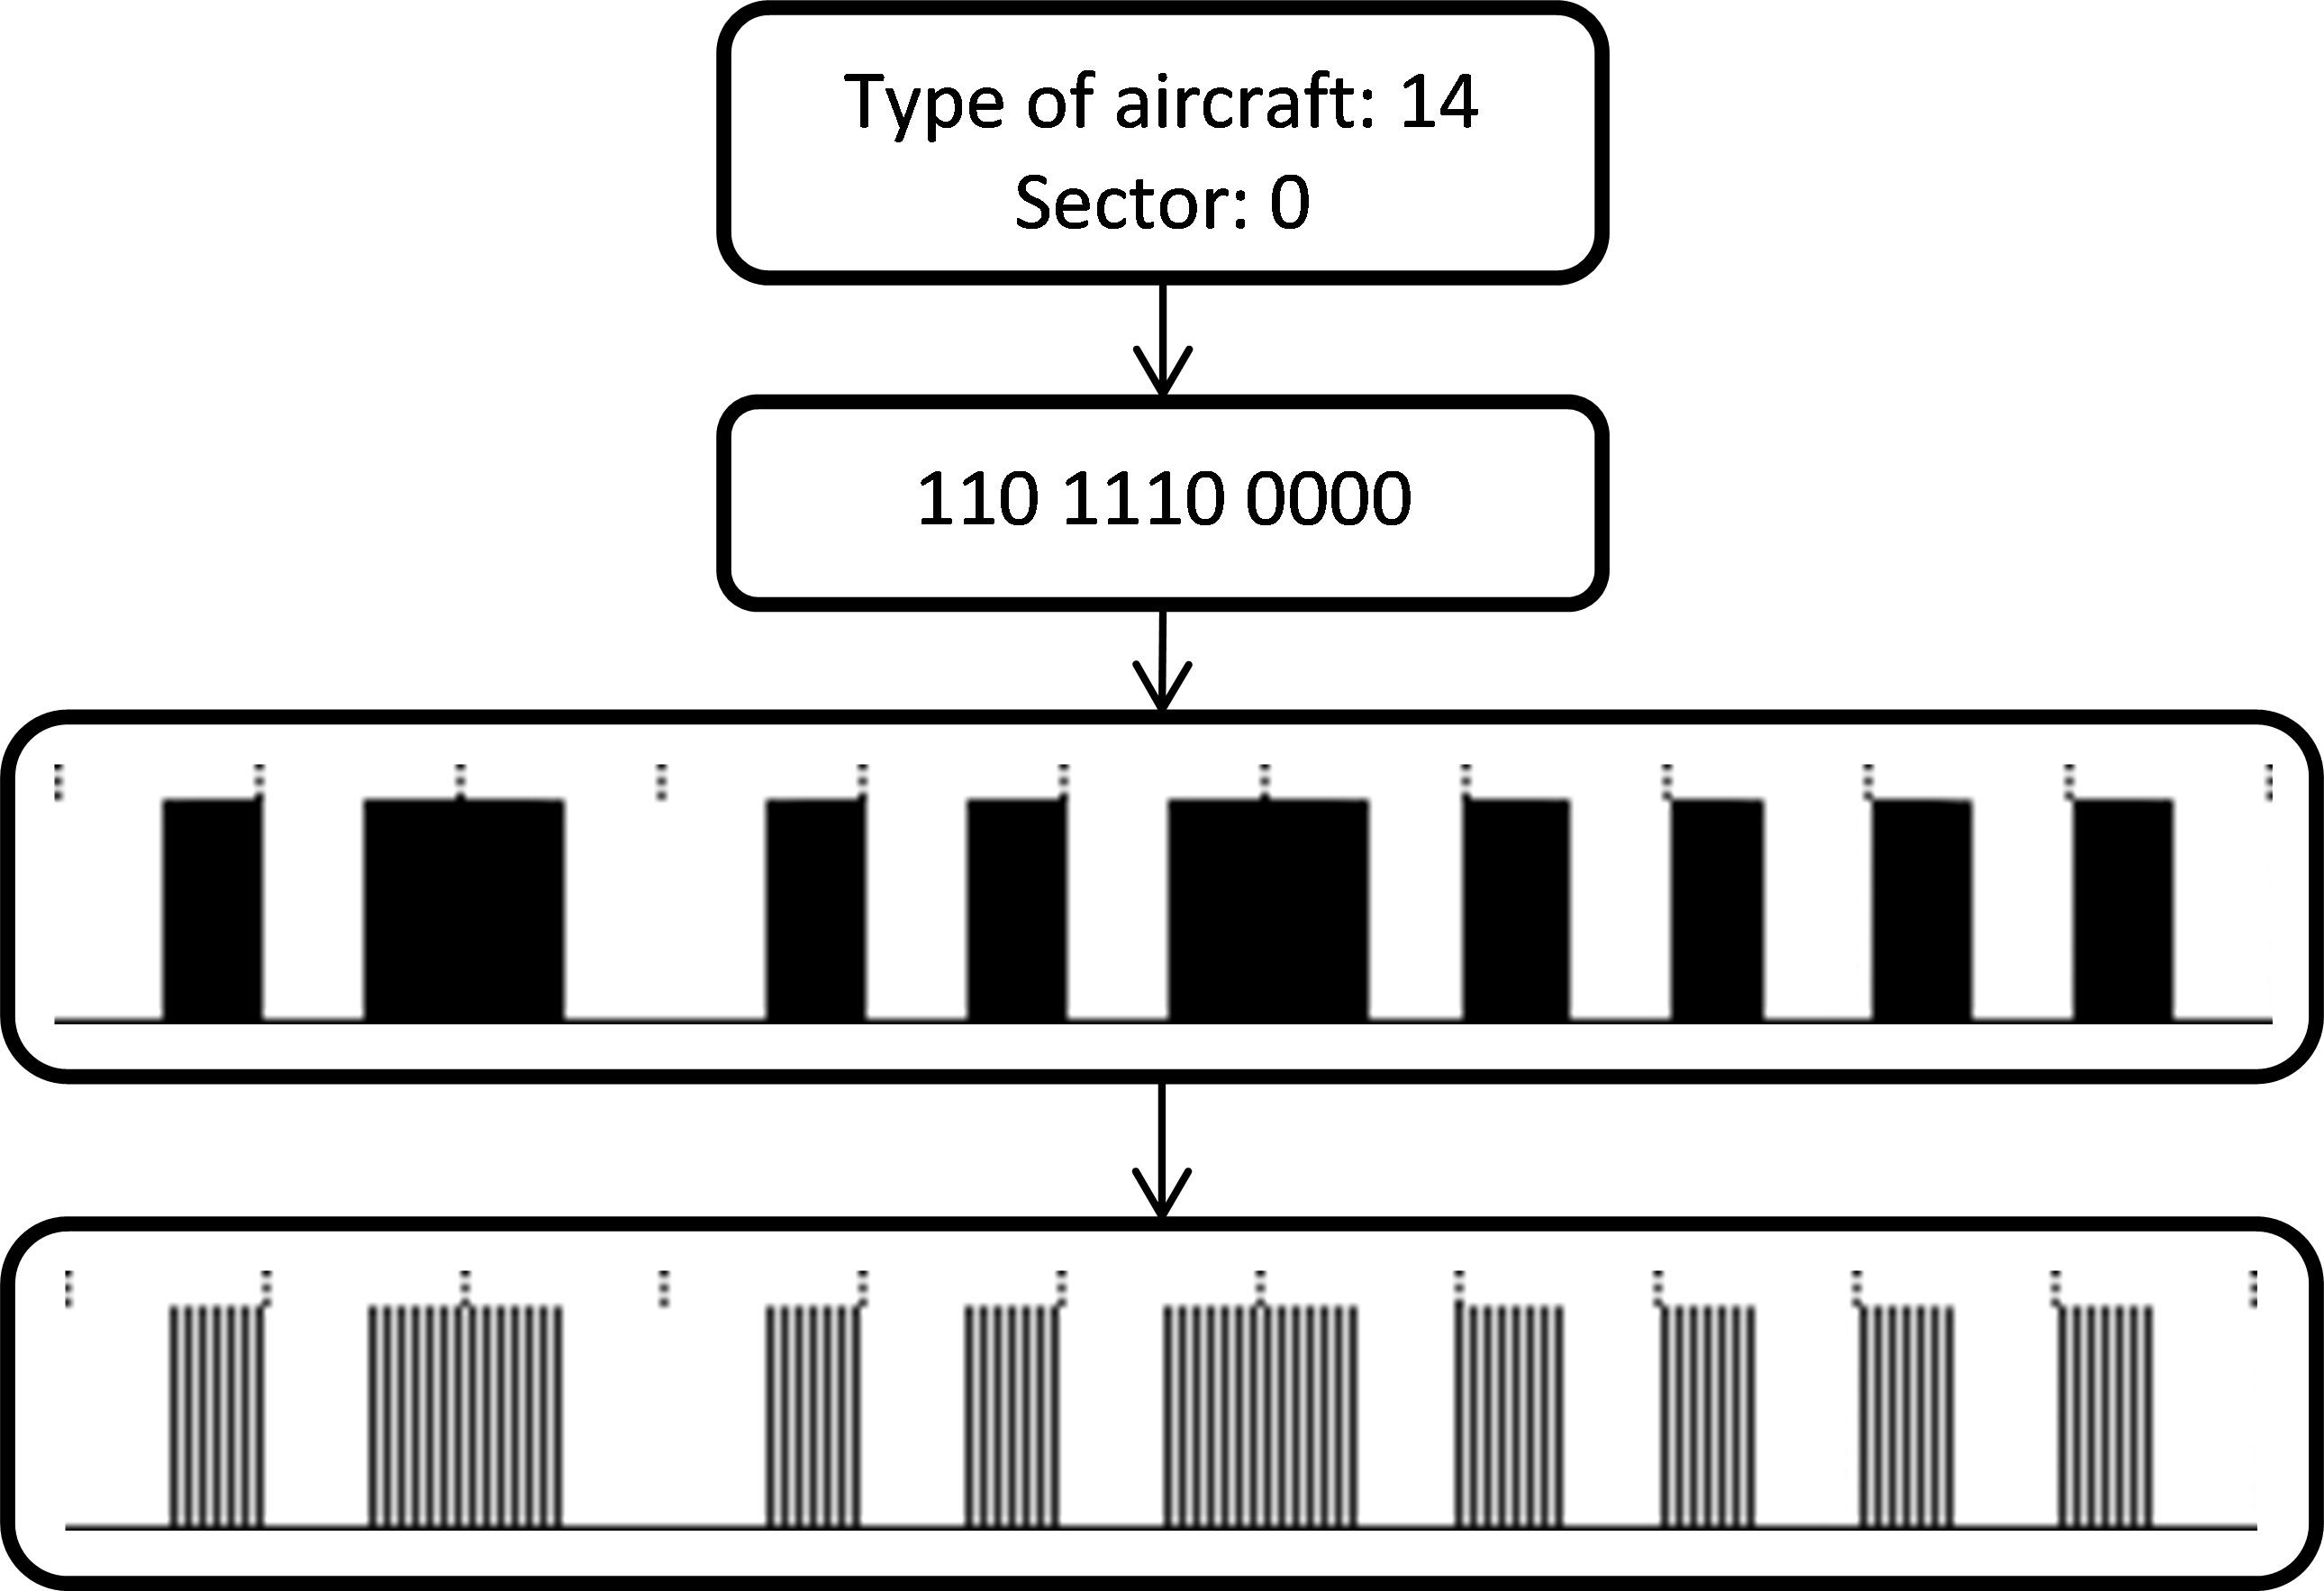
\includegraphics[width=0.8\textwidth]{Figures/messagecode.png}
  \caption[Process of Modulating the Transmitted Message]{Process of Modulating the Transmitted Message - signal not to scale}
  \label{fig:messagecode}
\end{figure}

When receiving, the microcontroller uses a Finite State Machine (FSM) to know which part of the message is expected to receive next. There are four different states, as can be seen in figure \ref{fig:IRspacestate}: Idle, where the microcontroller is waiting for a new message; Stop, in which a message has been fully received and is waiting to be decoded; SPACE, when a low level is being received; and finally MARK, where a high level is being received. The transitions are all represented in figure \ref{fig:IRspacestate}, where variables and functions are represented in lowercase (such as 'irdata' and 'timer') and constants are represented in capital letters ('RAWBUF' and 'GAP\_ TICKS'). The variable 'irdata' contains the received level, 'timer' is used to control the duration of each level, 'rawlen' is the number of entries received since the start of the message and 'decode' is the function that decodes the received message. In the used constants, 'GAP\_ TICKS' is used to control the minimum time between messages, 'RAWBUF' is the maximum length of the duration buffer, 'MARK' represents high level or bit '1' and finally 'SPACE' represents low level or bit '0'.\\
\begin{figure}[!htb]
  \centering
  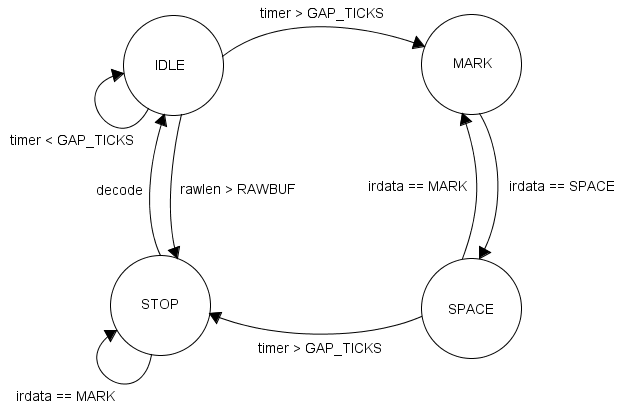
\includegraphics[width=0.9\textwidth]{Figures/IRspacestate.png}
  \caption[IRremote Reception Space State]{IRremote Reception Space State}
  \label{fig:IRspacestate}
\end{figure}

The entire code that allowed the interpretation for all the other protocols, except RC-5, was not needed and it occupied memory as well as processor during run-time, which would delay the reception and transmission of other messages. Because of this, all the unnecessary compiled code was removed.\\

The library was created to enable a single receiver or transmitter. To enable the number required for the prototype, several changes were made.\\
The first, which was necessary to allow several receivers, was to switch the \textit{irparams} structure, that saves everything needed for one receiver, to a vector of structures with length equal to the number of receivers. Then, the reception code was adapted to run for each receiver at a time.\\
The selected Arduino\texttrademark board has three available timers. The original code only used Timer 2 to enable both the transmission and the reception. As the transmission mode requires a timer to generate the PWM signal, while the reception only needs the timer to generate the reception interruptions, the two modes cannot operate with only one timer, or that timer would need to be configured every time it was used. Because Timer 0 is required for all code that manages time (delay, delayMicroseconds, etc...), the transmission was modified to use timer 1, while reception still uses timer 2.\\
As explained in section \ref{subsection:communication}, the signal is modulated using a 56 kHz frequency. The used IRremote library can only modulate signals with frequencies between 36 and 40 kHz, so it was modified for 56 kHz transmission, changing the setup of the timer to allow a faster operation.\\
While Timer 1 can be used to generate the required 56 kHz modulation, it can only output the signal to digital port 9 and so, a multiplexer is required to send the signal to the required 16 IR LEDs. 
By setting the Arduino's digital ports 2 to 5 with the appropriate signal (High or Low), the signal is only transmitted to the selected LED.\\

While studying the timings of the code, it was found that several commands were configuring the same options every cycle. To avoid this, several modifications were made: the configuration of the PWM generating timer (Timer 1) and the direction (output) of the digital ports used for transmission, 2-5 and 9, are now performed only once during the setup function, which only runs when the Arduino is turned on. \\ 

As referred in section \ref{subsection:pcontrolblink}, the Arduino\texttrademark Pro Mini also controls the Anti-Collision Light. The script 'morseaircraft.cpp', has the necessary code and only needs to be called before the setup, to generate the necessary variables (one of them is the type of aircraft in decimal), and once every loop to control the timing of the Morse Code transmitted by the Anti-Collision Light. More information about this script can be found in section \ref{subsection:pcontrolblink}. \\

With the changes stated in section \ref{subsection:solution}, the transmitted message is different from the original RC-5 and so, the transmission and decoding sections also had to be changed. In both sections (function IRsend::sendRC5 for transmission and function IRrecv::decodeRC5), the address bits were removed, the aircraft type was added and the command was replaced with the shorter identification of the transmitting sector.\\

Some important variables were introduced to control important timings in each cycle. The variable 'TX' changes the ratio between number of transmissions and receptions. For example, if 'TX' is 1, for each reception cycle there is one transmission cycle; if 'TX' is 5, there is one transmission cycle in every five reception cycles. 'A' changes the delay between each LED transmission in the same transmission cycle; 'REC' changes the delay before the reception cycle, which gives the receivers more time to receive a complete signal. Finally, there is 'RC5\_ T1' which is equal to half the duration of each transmitted bit. As the used PWM frequency is higher than the original RC-5, the "RC5\_ T1" time can be lowered to allow a higher transmission rate without reducing the number of PWM generated oscillations which are important for a successful reception.

The final code used with the prototype can be seen at https://github.com/MBSFonseca/SenseAndAvoidThesis.\\

\section{Material Testing}
\label{section:materialtesting}

Before building the prototype it was important to check the range and angular view of both the IR LED and the receiver.\\
To test the equipment's range and field of view, a test procedure was created (Test Procedure IR), as seen in section \ref{annex:irmaterial}, which consisted in transmitting several signals between two subsystems, the transmission and the receiver subsystems, at several ranges and angles.\\
%For the test procedure, a schematic was designed for each subsystem. The transmission subsystem, composed by an Arduino\texttrademark Uno, the IR LED, a MOSFET to control the LED with the Arduino\texttrademark, a resistor and a capacitor to control oscillations generated by the PWM signal, was connected according to figure \ref{fig:schematicIR1}. The receiving subsystem, which had the IR receiver, an Arduino\texttrademark Nano and an LED with a resistor that would blink when something was received.\\ , was connected according to figure \ref{fig:schematicIR2}.\\
%\begin{figure}[ht]
%  \centering
%  \subfigure[][]{
%    \label{fig:schematicIR1} 
%    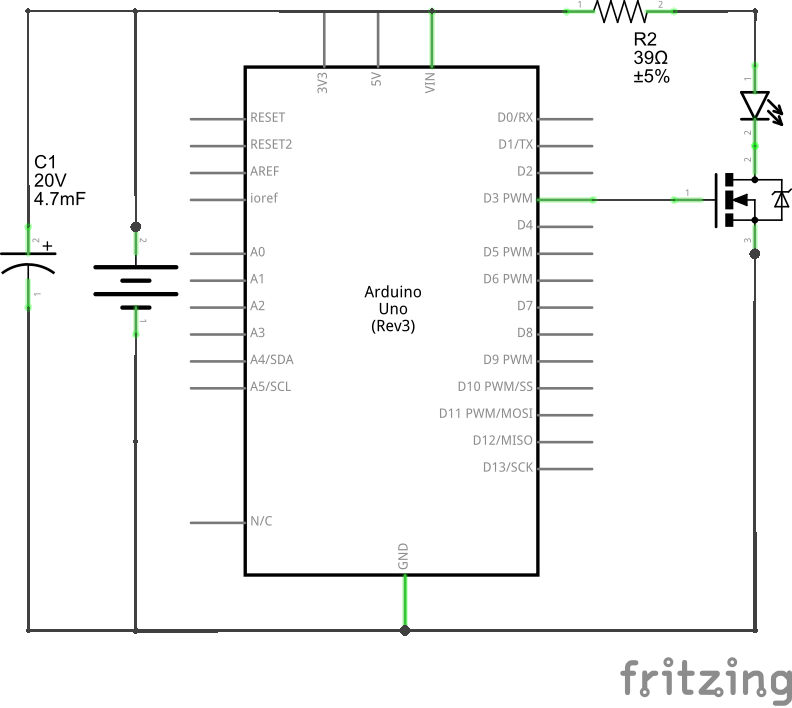
\includegraphics[]{Figures/esquemaled.png}
%  }
%  \hspace{8pt}
%  \subfigure[][]{
%    \label{fig:schematicIR2} 
%    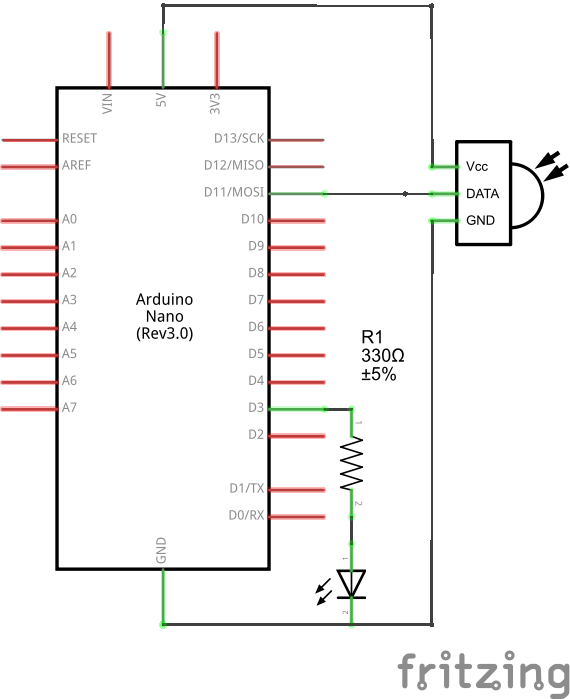
\includegraphics[]{Figures/esquemasensor.png} 
%  }
%  \caption[Schematic Diagram of each Subsystem for Test Procedure]{Schematic diagram of each subsystem for test procedure:
%			\subref{fig:schematicIR1} describes the Transmission subsystem;
%			\subref{fig:schematicIR2} describes the Receiving subsystem.}%
%  \label{fig:schmatics}%
%\end{figure}

The script 'TesteIRreceiver.ino' turns any LED connected to digital port 3 on, when any message is received by the receiver, and outputs the received value to the connected PC.
The script 'TesteIRsender.ino' transmits a message according to the adapted RC-5 protocol every half second. The message, at this time, still contained an address, which was always set to '14', and a command, which may be a '0', a '1' or a '2'.\\
To test the range of both subsystems and the field coverage of the receiving subsystem, an operator would place the transmission equipment on the 'X' mark in figure \ref{fig:ranges1}, and the receiving equipment at the 2 meters mark. After receiving any message, the operator would move the receiving subsystem in the direction of the other marks, perpendicular to the transmitter, until the maximum range was reached. Then the receiving subsystem would be rotated until a maximum angle of reception was reached.\\
\begin{figure}[!htb]
  \centering
  \includegraphics[width=0.70\textwidth]{Figures/ranges1.png}
  \caption[Distances and Positions for both Subsystems for test procedure 1]{Distances and Positions for both Subsystems for range and receiver's field coverage tests}
  \label{fig:ranges1}
\end{figure}

After that, to acquire the transmission subsystem's maximum angular view, the receiving subsystem would be placed in the 'X' mark, as showed in figure \ref{fig:ranges3}, and the transmission subsystem would be moved into the maximum range. A range of 50 m was assumed in the figure. There, the transmission equipment would be rotated until the maximum angular view was reached.\\
\begin{figure}[!htb]
  \centering
  \includegraphics[width=0.70\textwidth]{Figures/ranges3.png}
  \caption[Distances and Positions for both Subsystems for test procedure 2]{Distances and Positions for both Subsystems for transmission's field coverage tests}
  \label{fig:ranges3}
\end{figure}

The tests were repeated during day and nighttime. During daytime, the tests were repeated with a radiation filter on the receiving subsystem to reduce noise generated by the Sun.\\ 

A continuous power provider was used in the transmission subsystem in order to avoid fluctuations on the LEDs' intensity due to PWM oscillations and battery drainage.\\

The results were obtained with the conditions presented in figure \ref{fig:testirconditions}.\\

\begin{figure}[!htb]
  \centering
  \includegraphics[width=1\textwidth]{Figures/testirconditions.png}
  \caption[Conditions during IR test procedure]{Conditions during IR test procedure}
  \label{fig:testirconditions}
\end{figure}

The obtained results are presented in table \ref{tab:irtestsresults}. At night, the range for messages received correctly is 66 m, but it was found that, at 75 m, the receiver still received incomplete data.\\
\begin{table}[]
\centering
\caption{Results for IR test procedure}
\label{tab:irtestsresults}
\begin{tabular}{ccccc}
\hline
                                &              & \multicolumn{2}{c}{Day} & \multirow{2}{*}{Night} \\
                                &              & w/o filter  & w/ filter  &                        \\ \cmidrule(l){3-5}
\multicolumn{2}{c}{Range}                      & 20 m        & 30 m       & 66 m                   \\
\multirow{2}{*}{Field Coverage} & Transmission & 10\degree   & -          & 10\degree              \\
                                & Receiver     & 45\degree   & -          & 45\degree              \\ \hline
\end{tabular}
\end{table}

\section{Prototyping}
\label{section:prototypes}
As presented in section \ref{subsection:solution}, to provide a 360\degree angular coverage, the proposed configuration, showed in figure \ref{fig:irdiagram}, has 16 transmission sectors with one LED each and 4 reception sectors with one receiver each. \\
The first prototype was designed in Fritzing\texttrademark software, and it tried to have every element in a single perforated board. Adding to this, instead of using Darlington Transistor Arrays to control the LEDs, it used MOSFETs, the STB55NF06 in particular, used in the chapter \ref{chapter:passive}.\\ 
%The schematic and board for this prototype can be seen in figure \ref{fig:prototype1}. 
%\begin{figure}[!htb]
%  \centering
%  \subfigure[][]{
%    \label{fig:prototype1schematic} 
%  	\includegraphics[width=0.45\textwidth]{Figures/Prototype1_Esquema.png}
%  }
%  \hspace{8pt}
%  \subfigure[][]{
%    \label{fig:prototype1board} 
%    \includegraphics[width=0.45\textwidth]{Figures/Prototype1_bb.png} 
%  }
%  \caption[First Prototype]{First Prototype:
%			\subref{fig:prototype1schematic} schematic; and,
%			\subref{fig:prototype1board} board.}%
%  \label{fig:prototype1}%
%\end{figure}
%As can be seen in figure \ref{fig:prototype1board}, 
The designed board had to be too wide due to the amount of elements required, with the used MOSFET occupying most of the space. Another problem was the amount of wires required for the connections. As a solution for this problem, a printed circuit was planned but, due to the high number of connections that exited the multiplexer and the Arduino\texttrademark board, the board would have to be double-sided, which is much more complex or expensive to manufacture. Finally the program used to design the board didn't have all the components required and it didn't offer enough tools to correctly position each component.\\

The solution for most problems was to split the equipment into two separate boards: one responsible for transmission and another for reception.\\
Because the previous used program, Fritzing\texttrademark , did not allow to exactly place each element where it was required, a different one was used to design the second version, Eagle\texttrademark .\\

As the prototype is intended to be assembled by each user, it should be easy to manufacture or not expensive to buy already printed. With this in mind, the printed circuit board was designed with thick connections and wide spacing between them, as can be seen in figure \ref{fig:prototype2}.\\
\begin{figure}[!htb]
  \centering
  \subfigure[][]{
    \label{fig:transmitterboard} 
    \includegraphics[width=0.45\textwidth]{Figures/transmitterboard.png}
  }
  \hspace{8pt}
  \subfigure[][]{
    \label{fig:receiverboard} 
    \includegraphics[width=0.45\textwidth]{Figures/receiverboard.png}
  }
  \caption[Second Prototype]{Second Prototype:
			\subref{fig:transmitterboard} transmitter board; and,
			\subref{fig:receiverboard} receiver board.}%
  \label{fig:prototype2}%
\end{figure}

Both boards were printed and the excess copper removed using iron chloride, as shown in figure \ref{fig:pcbmaking}. There were some problems with connections that did not transfer to the copper, and so some connections had to be tinned.\\
%Even so, there were some difficulties found during manufacture:
%\begin{itemize}
%\item A laser printer is required
%\item First board designed with the selected software (Eagle\texttrademark )
%\item Printer's software changed the size of the board
%\item Correctly drill the required holes
%\item Soldering SMDs
%\item Cables used to connect boards were too thick and rigid
%\item Several printed connections did not transfer correctly to copper and disappeared 
%\end{itemize}

\begin{figure}[!htb]
  \centering
  \subfigure[][]{
    \label{fig:pcbcopper} 
    \includegraphics[width=0.3\textwidth]{Figures/pcb2.png}
  }
  \hspace{8pt}
  \subfigure[][]{
    \label{fig:pcbacid1} 
    \includegraphics[width=0.3\textwidth]{Figures/pcb1.png} 
  }\\
  \subfigure[][]{
    \label{fig:pcbacid2} 
    \includegraphics[width=0.3\textwidth]{Figures/pcb4.png}
  }
  \hspace{8pt}
  \subfigure[][]{
    \label{fig:pcbend} 
    \includegraphics[width=0.3\textwidth]{Figures/pcb5.png} 
  }
  \caption[PCB printing process]{PCB printing process:
			\subref{fig:pcbcopper} printed image transferred to copper;
			\subref{fig:pcbacid1} iron chloride reacting with copper;
			\subref{fig:pcbacid2} iron chloride reacting with copper; and,
			\subref{fig:pcbend} finished boards.}%
  \label{fig:pcbmaking}%
\end{figure}

After finishing the boards, the elements were soldered with special attention to the SMD components, the cables that connect the boards were manufactured and two prototypes were assembled, as shown in figure \ref{fig:twoprototypes}.\\
\begin{figure}[!htb]
  \centering
  \includegraphics[width=0.8\textwidth]{Figures/twoprototypes.png}
  \caption[Finished prototypes]{Finished prototypes}
  \label{fig:twoprototypes}
\end{figure}

To protect the prototypes and to decrease the angular view of the IR receivers, a 3D printed box was created. The box is composed of three parts, so that the prototype can be assembled inside the box.\\
As each receiver is able to receive beyond the angular view of 90\degree , the reception sectors for each receiver were increased to 130\degree . This increase in the angular view creates four virtual sectors, where the signal is received by two receivers.\\
The technical drawings of the created design can be seen in \textbf{\# Annex reference here \#}.
After printing, the pieces were also painted black.\\
The final result can be seen in figures~\ref{fig:printedbox2}--\subref{fig:printedbox3}.\\

\begin{figure}[!htb]
  \centering
  \subfigure[][]{
    \label{fig:printedbox2} 
    \includegraphics[width=0.45\textwidth]{Figures/printedbox2.png}
  }
  \hspace{8pt}
  \subfigure[][]{
    \label{fig:printedbox3} 
    \includegraphics[width=0.45\textwidth]{Figures/printedbox3.png} 
  }\\
  \caption[3D Printed Box]{3D printed box:
			\subref{fig:printedbox2} printed parts; and,
			\subref{fig:printedbox3} assembled box.}%
  \label{fig:printedbox}%
\end{figure}

The assembled product is shown in figures~\ref{fig:irprototype1}--\subref{fig:irprototype2}.\\

\begin{figure}[!htb]
  \centering
  \subfigure[][]{
    \label{fig:irprototype1} 
    \includegraphics[width=0.45\textwidth]{Figures/irprototype1.png}
  }
  \hspace{8pt}
  \subfigure[][]{
    \label{fig:irprototype2} 
    \includegraphics[width=0.45\textwidth]{Figures/irprototype2.png} 
  }\\
  \caption[Assembled IR Sense and Avoid Prototype]{Assembled IR sense and avoid prototype:
			\subref{fig:irprototype1} top view; and,
			\subref{fig:irprototype2} side view.}%
  \label{fig:irprototype}%
\end{figure}

The total acquisition cost is \euro{37,54} which include \euro{10} for miscellaneous items, such as cables, connectors and plastic for the printed box.\\

\subsection{ISR's quadcopter}
\label{subsection:IRpisr}
The created prototype was then adapted to a quadcopter. \\
The used quadcopter has a Nvidia Jetson Tk1 onboard, which is responsible for the high level control. This board would be responsible to avoid collisions, receiving data from the prototype through USB serial communication.\\
The only required connections between the aircraft and the prototype are a USB serial port, used to establish communication between the prototype and the Nvidia board, and two cables connected to the aircraft's power distribution board in order to power up the prototype.\\
The quadcopter can be seen in figure \ref{fig:irprototype3} with the prototype fixed on top.\\

\begin{figure}[!htb]
  \centering
  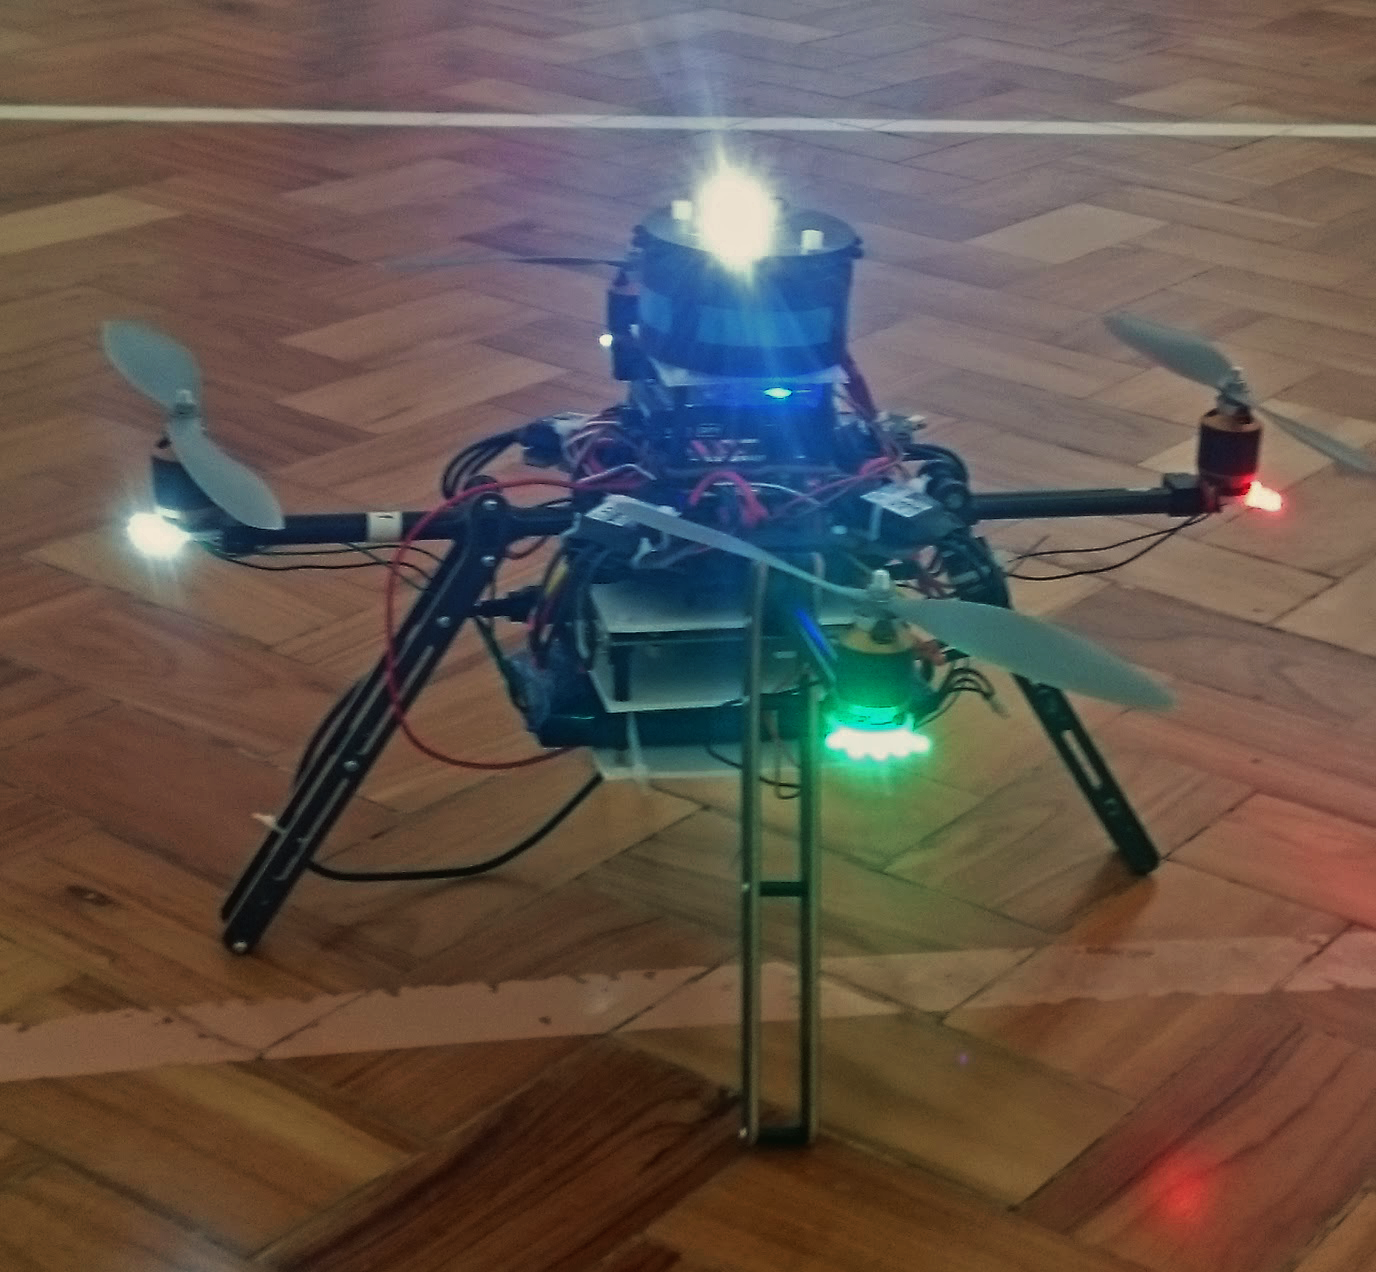
\includegraphics[width=0.6\textwidth]{Figures/irprototype3.png}
  \caption[IR Sense and Avoid Prototype Assembled on Quadcopter]{IR sense and avoid prototype assembled on quadcopter}
  \label{fig:irprototype3}
\end{figure}

\section{Prototype Testing}
\label{section:prototypetest}
\subsection{Time Variables Optimization}
\label{subsection:opt}
Before testing the prototypes, the four variables ('TX', 'A', 'REC' and 'RC5\_ T1') that control important times in each cycle had to be optimized. To do this, an automatic test was designed. Two prototypes would run the given values for 60 seconds and the number of receptions during each test would be saved.\\
As the variable 'RC5\_ T1' can not be changed without compiling the code, the test would only change the other three variables, with the 'RC5\_ T1' being changed by hand between tests.\\
Each prototype would be connected to a different computer and laboratory power supplies, and would be place 10 m apart without obstacles between them.  The developed code would be loaded into each Arduino\texttrademark board, so that the prototype would wait for the variables that each pc would send. After the setup cycle, the code is equal to the normal Sense and Avoid prototype.\\

To enable synchronization between both prototypes, a Socket server and client were developed in Python. One computer would run the server and the other the client.\\
The server script waits to receive 'TX', 'A' and 'REC' from the client and then sends this information to the connected prototype. It then allows the prototype to run normally until the client tells him to stop and sends the new values for the variables, which the server then sends to the prototype again. In the client side, the script first changes the tested variables, sending them to the server and to its connected prototype. After one minute, it stops the communication with the prototype, tells the server to do the same, saves the variables' values and the number of receptions into a file and starts again with different values.\\

The tested values were:
\begin{itemize}
\item 'TX' - 1, 5, 10, 15, 20
\item 'A' - 1, 3, 5, 10
\item 'REC' - 10, 20, 40, 60, 100
\item 'RC5\_ T1' - 100, 200, 300, 500, 700, 889
\end{itemize}

\subsection{Blind zones}
\label{subsection:blindzones}
In order to check if the prototypes had blind zones in transmission or reception, a test was prepared.\\
To check for blind zones in transmission, both prototypes are set on tripods to avoid reflections from the ground. Then, one prototype is connected to the PC and battery, while the second prototype is placed at the tested distance, only connected to the battery, and is able to rotate. With both prototypes working, the second prototype is rotated in 5\degree intervals, with a pause of 5 seconds between rotation, until the 360\degree are reached. At the end, the number of receptions shows the angular transmission quality.\\

To check for blind zones in reception, both prototypes are set on tripods to avoid reflections from the ground. Then, one prototype is connected to the PC and battery, while the second prototype is placed at the tested distance, only connected to the battery. With both prototypes working, the first prototype, which is connected to the PC, is rotated in 5\degree intervals, with a pause of 5 seconds between rotation, until the 360\degree are reached. At the end, the number of receptions shows the angular reception quality.\\

The tests were repeated at ranges of 7, 9 and 11 meters.\\

\subsection{Ranges}
\label{subsection:ranges}
In order to check the maximum range of the prototype, a test procedure was designed.\\
With one prototype fixed, the other would move away in a straight line, perpendicularly to the fixed prototype, until the maximum range was found. The test would be repeated during day and nighttime, inside a building and outside.\\ 

As it was found that the receivers would saturate with the selected resistors, due to high radiant intensity, another two resistors with lower resistances (56 and 82 $\Omega$) were tested indoors during daytime.\\
Using equation \eqref{eq:ohm2} and figure \ref{fig:ledintensity} again, we can calculate the LED's forward current and radiant intensity with the new resistors. The results are shown in table \ref{tab:ledintensity2}.\\
\begin{table}[]
\centering
\caption[Forward Current and Radiant Intensity of IR LED with new Resistors]{Forward Current and Radiant Intensity of IR LED with new Resistors}
\label{tab:ledintensity2}
\begin{tabular}{@{}ccc@{}}
\toprule
                     & Forward Current (mA) & Radiant Intensity (mW/sr) \\ \cmidrule(l){2-3}
56 $\Omega$ Resistor & 136.6                & 200                       \\
82 $\Omega$ Resistor & 93.3                 & 150                       \\ \bottomrule
\end{tabular}
\end{table}

Adding to this, a filter was applied to the receivers to reduce ambient noise and the tests were repeated.\\

\subsection{Maneuvers}
\label{subsection:maneuvers}
In order to test the designed prototypes in important situations for collision avoidance, a test procedure was planned, as can be seen in section \ref{annex:maneuvers}.\\
Several configurations would be evaluated, as shown in figures~\ref{fig:configheadon}--\subref{fig:configovertaking}, beginning with static tests of each situation, followed by non-static tests which tried to simulate the correct avoidance maneuvers for each situation.\\ 

\begin{figure}[!htb]
  \centering
  \subfigure[][]{
     \includegraphics[width=0.25\textwidth]{Figures/VL-Rules3.jpg}
     \label{fig:configheadon}
  }\hspace{3pt}
  \subfigure[][]{
     \includegraphics[width=0.33\textwidth]{Figures/VL-Rules4.jpg}
     \label{fig:configconverging}
  }\hspace{3pt}
  \subfigure[][]{
     \includegraphics[width=0.25\textwidth]{Figures/VL-Rules5.jpg}
     \label{fig:configovertaking}
  }\\
  \caption[Maneuvers Test's Configurations \citep{Planefinder2012}]{Maneuvers Test's Configurations \citep{Planefinder2012}:
			\subref{fig:configheadon} - head on approach;
			\subref{fig:configconverging} - converging approach; and,
			\subref{fig:configovertaking} - overtaking approach.}%
  \label{fig:configurations}
\end{figure}

\subsection{ISR drone}
\label{subsection:IRisrdrone}

In order to test the designed prototypes with an aircraft, a test procedure was planned, which can be seen in section \ref{annex:sas}.\\
The same configurations of section \ref{subsection:maneuvers} would be tested.\\ 

The Nvidia on-board the aircraft was programmed to start a serial communication with the prototype at start up, and log all the data received into a file with the time stamp.\\
As a first test, one prototype would be fixed on top of a quadcopter and the other placed on top of a tripod. The aircraft would then move as described in the test procedure, so that detection data would be stored.\\
Due to time restrictions and problems with the used quadcopter's batteries, the test could not be successfully completed and no results were collected.\\
